\documentclass[9pt,a4j,twocolumn]{jsarticle}
\usepackage[dvipdfmx]{graphicx}
\usepackage{ascmac}
\usepackage{txfonts}
\usepackage{float}
\usepackage{cite}

\setlength{\topmargin}{-3cm}
\setlength{\textheight}{29.5cm}
\setlength{\textwidth}{20.0cm}
\setlength{\oddsidemargin}{-0.9cm}
\setlength{\evensidemargin}{-0.9cm}
\setlength{\baselineskip}{0.5cm}
\renewcommand{\baselinestretch}{0.865}

\title{
    Computer Networking\\
    A Top-Down Approach pp.144-169
}
\author{
    %トップダウン・アプローチの作者
    James F. Kurose, Keith W. Roth
    \\\\
    情報工学科3年 寺岡研究室\\
    学籍番号 61619027 名前 安森涼
}
\date{2019年 2月 14日}
\begin{document}
\maketitle

\section{Peer to Peer アプリケーション}
Web, Email, DNSのようにクライアントとサーバの関係にあるものは基盤サーバ側に信頼が必要である.一方でPeer to Peer(P2P)アプリケーションは基盤サーバ側に信頼を必要としない.その代わり,ピアという断続的につながっているホストの組が必要で,これはサービスプロバイダではなく,ユーザのデスクトップやノートパソコン間で提供されるものである.この節では,P2Pによく適している二つの異なるアプリケーションを説明する.一つ目がファイル分配で単一のソースから多くのピアにファイルを送信するものである.この例として,最も一般的なP2Pファイル分配プロトコルであるBitTorrentを紹介する.二つ目が分散データベースで,これは巨大なピアの共同体により配信されるデータベースである.ここでDatabase Hash Tables (DHT)について述べる.
\\
\subsection{ファイル分配}
P2PではLinux OSのアップデート,ソフトウェア,MP3音楽ファイル,MPEGビデオファイルなどの大容量のファイルを単一のサーバから多数のホストに送ることを考える.クライアントサーバ構造でのファイル分配ではサーバがピアに大きなファイルを送る.この際,サーバのチア息を大きく占有してしまうという問題がある.P2P構造のファイル分配ではピア側のどの部分でも再分配できる.そのためサーバの帯域を占有せずにファイルの送信が可能である.WebブラウザがHTTPを形成しているように,BitTorrentがプロトコルを形成している.
\\
\subsubsection{スケーラビリティ}
スケーラビリティとは利用者や仕事の増大に適応できる能力度合いのことである.これを説明するのに後述の図\ref{fig:file_distribution}のようなピアとサーバがリンクでつながっている構造を考え,P2P構造とクライアントサーバ構造で,全てのピアへの送信にかかる時間を比較する.ここでサーバのアップロード速度を$u_s$,i番目のピアのアップロード速度を$d_i$,i番目のピアのダウンロード速度を$d_i$,ファイルの大きさを$F$,送信するピアの数を$N$とする.本文章では$N$個全てのピアがダウンロードするのにかかる時間を元にスケーラビリティを比較する.この時間を以降分配時間と呼ぶ.また,条件を公平にするために,仮定としてインターネットが十分な帯域を保持していると考え、サーバとクライアントが他のネットワークに参加していないと考える.
\begin{figure}[tb]
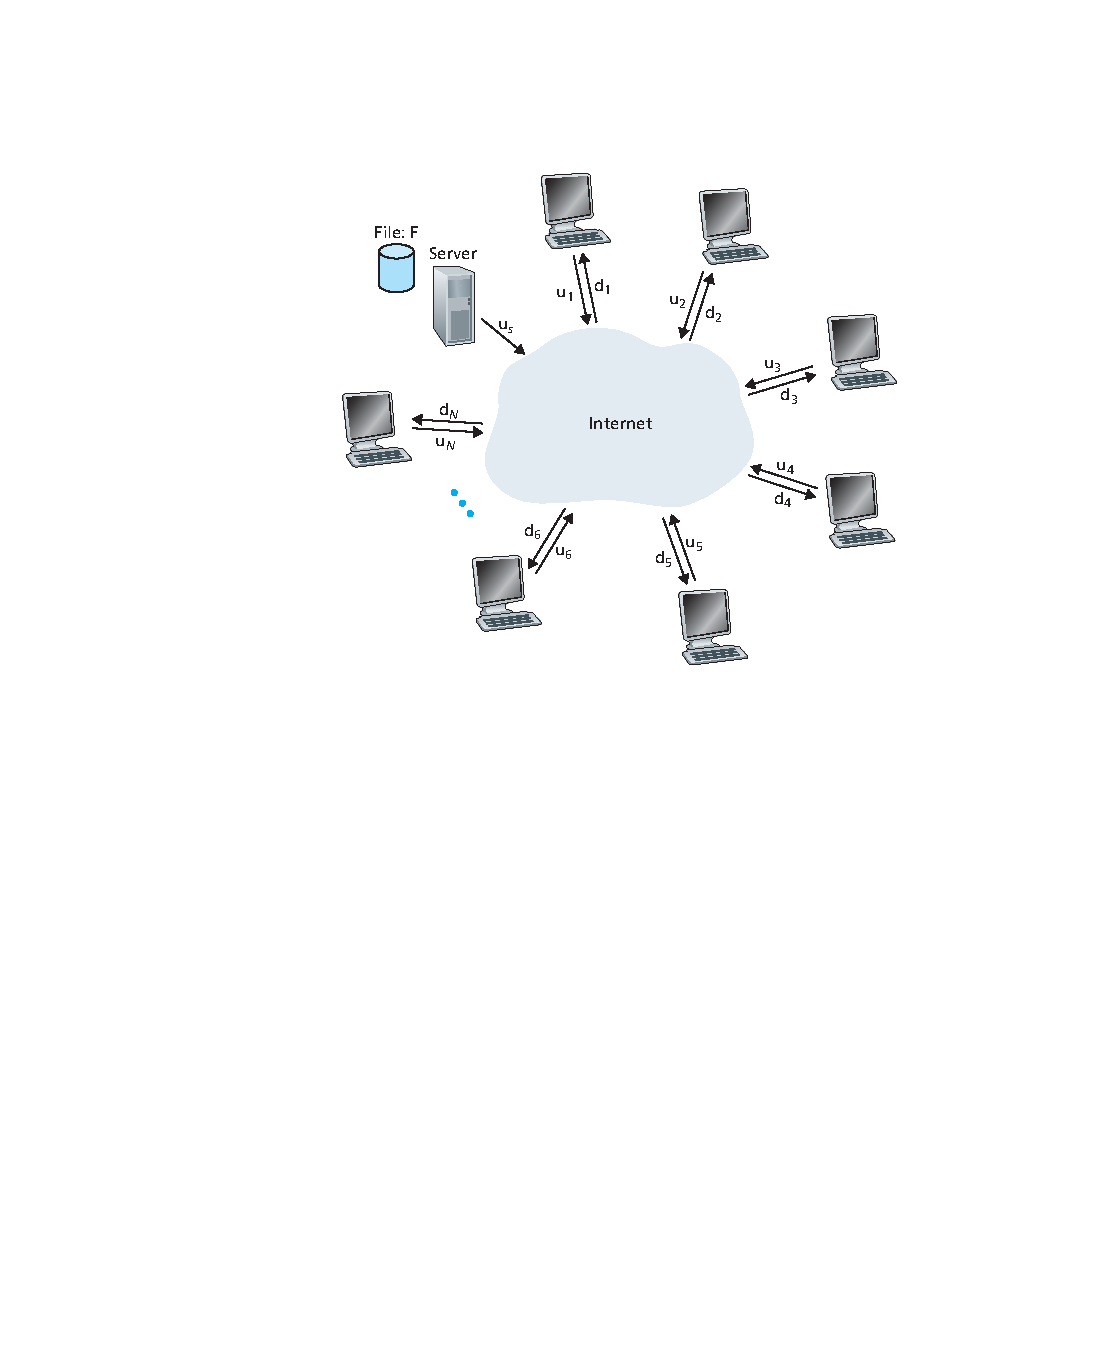
\includegraphics[width=10cm,pagebox=cropbox,clip]{FileDistribution.pdf}
 \caption{ピアとサーバがリンクでつながっている構造}
 \label{fig:file_distribution}
\end{figure}
まず,クライアントサーバ構造について分配時間を${D}_{cs}$と考える.サーバがピアへ送信することとピアが受信すること2つの面を考える.以降,データの容量の単位をbit,時間の単位を(hour),送信速度を (bit/hour)として考える.まず,前者について,送信するデータの総容量は$NF$であり,送信速度は前述の通り,$u_s$である.ゆえに,送信時間は$NF/u_s$で表される.続いて,後者については多数のピアの中で最短の受信速度は${d}_{min} = \min \{d_1 \sim d_N\}$であるため,受信時間は$F/{d}_{min}$で表される.これらより送信にかかる時間は前述の2側面のうち長い方なので
\begin{equation}
{D}_{cs}=\max \{ \frac{NF}{u_s}, \frac{F}{{d}_{min}} \}
\label{eq:cs}
\end{equation}
と表される.これより$N$が十分に大きいときに$N$の大きさに伴い線形に増加することがわかる.

続いて,P2P構造の分配時間を$D_p$と考える.サーバのピアへの送信にかかる時間,ピアの受信時間とシステム全体の送信能力から考える時間の3つの観点から考える.まず,1つ目の観点において,サーバは1度だけアクセスリンクに送信するので最短の送信にかかる時間は$F/u_s$である.また,2つ目の観点についてはサーバクライアント構造と同様に$F/{d}_{min}$である.最後の観点について,サーバとここのピアノ送信能力の和とシステム全体の送信能力は同等と考えられる.送信するデータの総容量は$NF$,送信速度は$u_s + \sum^{N}_{i=1}$ である.ゆえにこの観点からは少なくとも分配時間が$\frac{NF}{u_s + \sum^{N}_{i=1}}$と表される.故に分配時間が
\begin{equation}
D_p = \max \{ \frac{F}{u_s}, \frac{F}{{d}_{min}}, \frac{NF}{u_s + \sum^{N}_{i=1}} \}
\label{eq:p2p}
\end{equation}
と表される.

式(\ref{eq:cs}),(\ref{eq:p2p})より送信時間の比較を行う.ピアの送信速度を一律$u$ (bit/hour),$F/u + 1$ (hour),$u_s = 10u$,${d}_{min} \geqq u_s$とすると図
\ref{fig:graph}より常にP2Pの送信時間が短く,$N$がどんな値でもP2Pの送信時間が1時間未満であることがわかる.
\begin{figure}[tb]
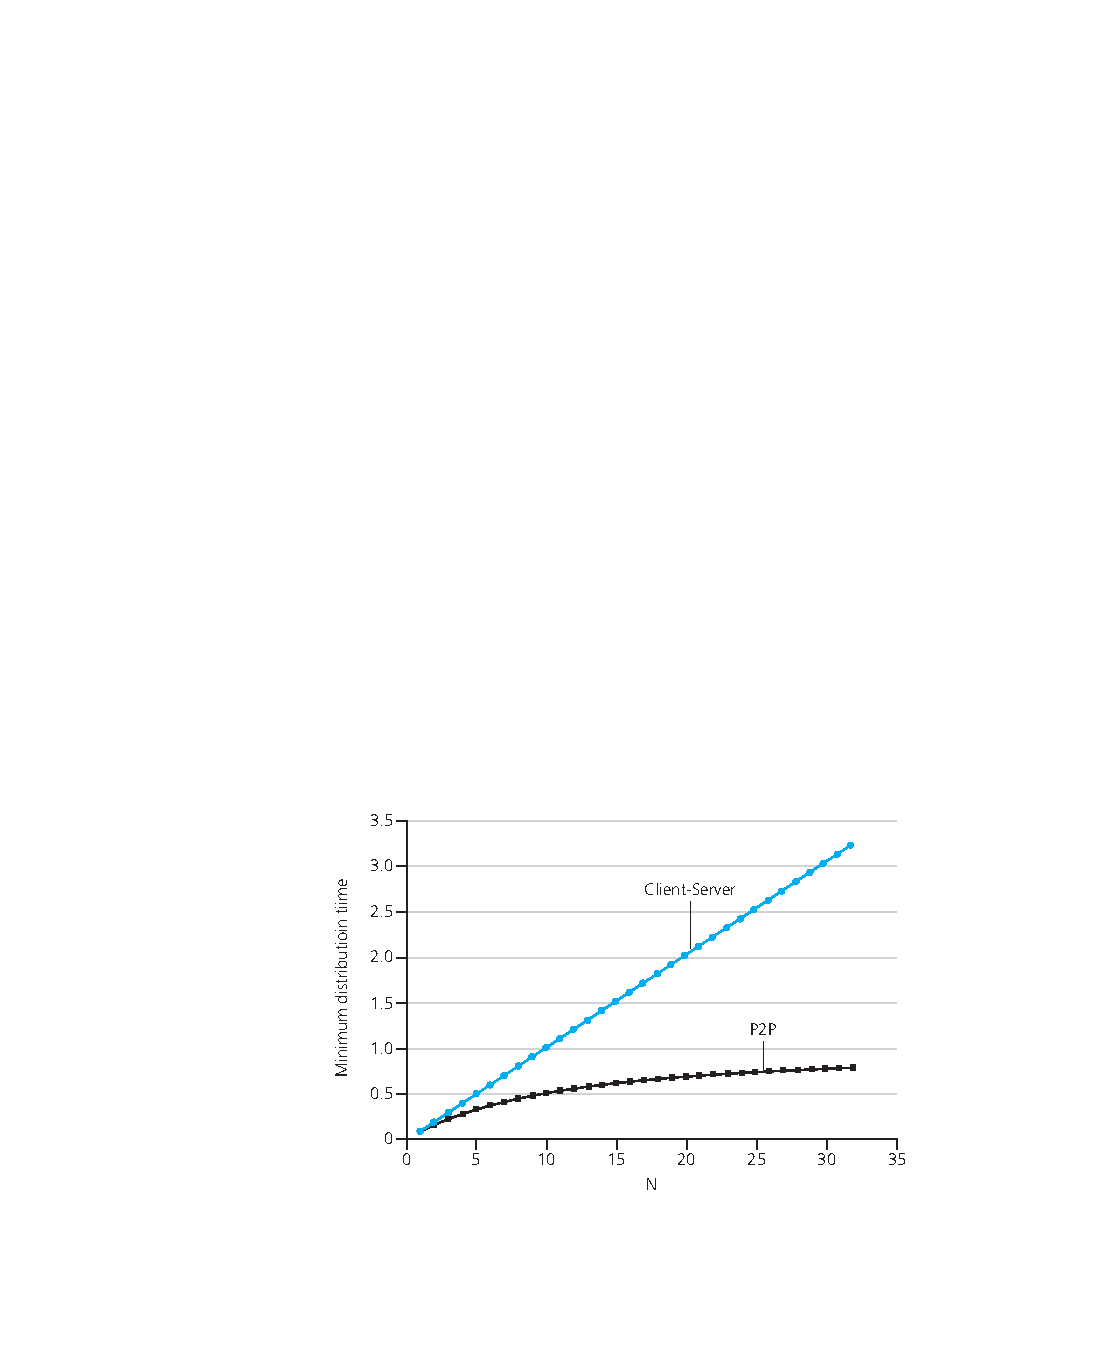
\includegraphics[width=10cm,pagebox=cropbox,clip]{graph.pdf}
 \caption{クライアントサーバ構造とP2P構造の送信時間の比較}
 \label{fig:graph}
\end{figure}
\\
\subsubsection{BitTorrent}
続いてBitTorrentについて記述する.これはファイル分配における有名なP2Pプロトコルである.このプロトコルの名前になっているトレントというものはあるファイルの分配に参加している全てのピアの集合である.このトレント内のピアがファイルを分割したチャンクを受信し,ピアが受信すると同時にチャンクの送信も行う.ピアが全体のファイルを取得するとトレントを離脱する,またはトレントに残り他のピアにチャンクを送信する.また,トレント内のピアの特徴としていつでもトレントの離脱と加入が可能である.また,トレントがトラッカというノードを所持していることで,トラッカはトレントに加入したピアのIPアドレスを保持することで,トレント内のピアの存在の是非をトラッカに定期通知することでトレント内のピアの追跡を行うことができる.例えばAliceというピアを考慮すると,Aliceは他のピアと通信を行い,トラッカから通信に成功したピアノIPアドレスを取得する.このように通信に成功したピアを以降隣接ピアと呼ぶ.Aliceは隣接ピアの通信確立を繰り返し行い,隣接ピアが所持しているチャンクのリストを入手し,これを元に所持していないチャンクの要求をする.このチャンクの要求方法として,rarest firstとunchokedがある.前者は隣接ピアに存在する複製が少ない貴重なチャンクから要求を行う.隣接ピアの中でコピーされている回数が少ないものから貴重なチャンクを判断する.後者はデータの割合が高いペア(以下unchokedと示す)を4つ選択肢,この4つのピアに自身のチャンクを送信し,一定間隔ごとに新しい相手を探し,チャンクを送信を繰り返す.他のピアのunchokedの1つとなったらチャンクを取得できる.これによりトレント内のチャンクのコピーの個数が一定に近づく.
\\
\subsection{分散データベース}
\subsubsection{Distributed Hash Tables (DHT)}
続いてDHTについて述べる.これは(キー,値)のペアを持つ単純なデータベースでP2P構造は多数のピアにペアの一部を保存することでどのピアにも特定のキーで問い合わせや挿入が可能になるものである.ピアに
nbit表現でIDを割り振り,キーにも同じ範囲の整数でIDの割り振りを実施する.そしてキーを自身と最も近いIDを持つピアに格納をすることでペアを保存している.元々のキーが数字以外の場合はハッシュ化し,数値化を行う.ハッシュ化は7章で取り扱うため深くは述べないが,これに用いられるハッシュ関数は多対1関数であるため,出力が等しくなることがあるが,出力が同じ場合の入力の差は非常に少ないので同じものとみなすことができる.キーに自身と最も近いピアの選択を行うさい,全てのピアを探索するのは不可能である.本レポートでは円形DHTについて説明する.
\\
\subsubsection{円形DHT}
円形DHTとは図\ref{fig:circular_dht}のように円形に配置されたピアのことである.それぞれのピアは前後のピアの情報を保持し,ピアにキーの情報がないとき,次のピアを調査することで探索を行うものである.ピアが自由に参加離脱することから削除挿入において配列より計算が早いリストを利用しており,リストの途中の要素からたどり始めたとしても、リスト全体を一周することが容易であるため循環リストを利用し,突然の挿入削除に対して対応できる双方向型のリストを採用している.例えば図\ref{fig:circular_dht}のように[0,15]であるこの中に8つのピアが存在し,そのIDを1,3,4,5,8,10,12,15とする.今回,ピア3から探索をし,挿入するペアのキーが11とする.探索をID3,4,5,8,10,12の順に行う.今回は自身に続く最も近いピアを選択するという規則にすると,12のIDが割り振られたピアにペアを格納することとなる.この方式によりピアは2つの隣接ピアの情報のみ保持する.このため保持する情報を削減することができる.ただしこの方法には欠点があり,ノード数を$N$とすると最悪の場合$N$ノード全てに問い合わせを行い,平均で$N/2$ノードに問い合わせを行う必要がある.このように保持する隣接ピアの情報の個数と問い合わせの回数はトレードオフの関係にある.この問い合わせの回数を減らすために図\ref{fig:circular_dht_with_shortcuts}のようにショートカットを追加することが必要である.
\\
\begin{figure}[tb]
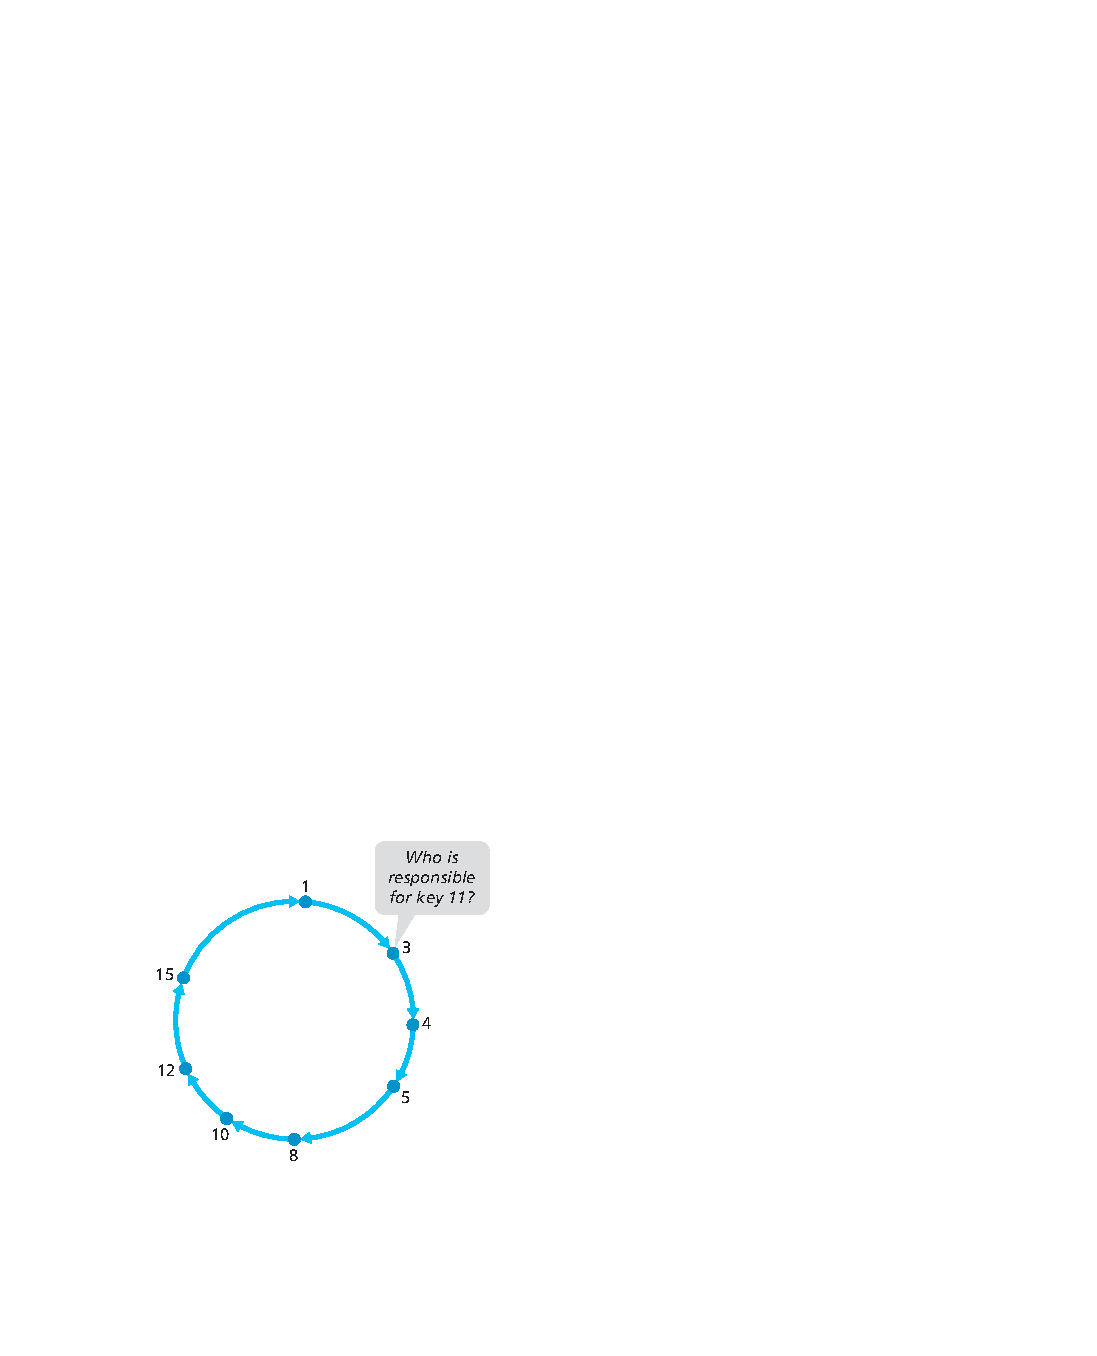
\includegraphics[width=10cm,pagebox=cropbox,clip]{CircularDHT.pdf}
 \caption{円形DHT}
 \label{fig:circular_dht}
\end{figure}

\begin{figure}[tb]
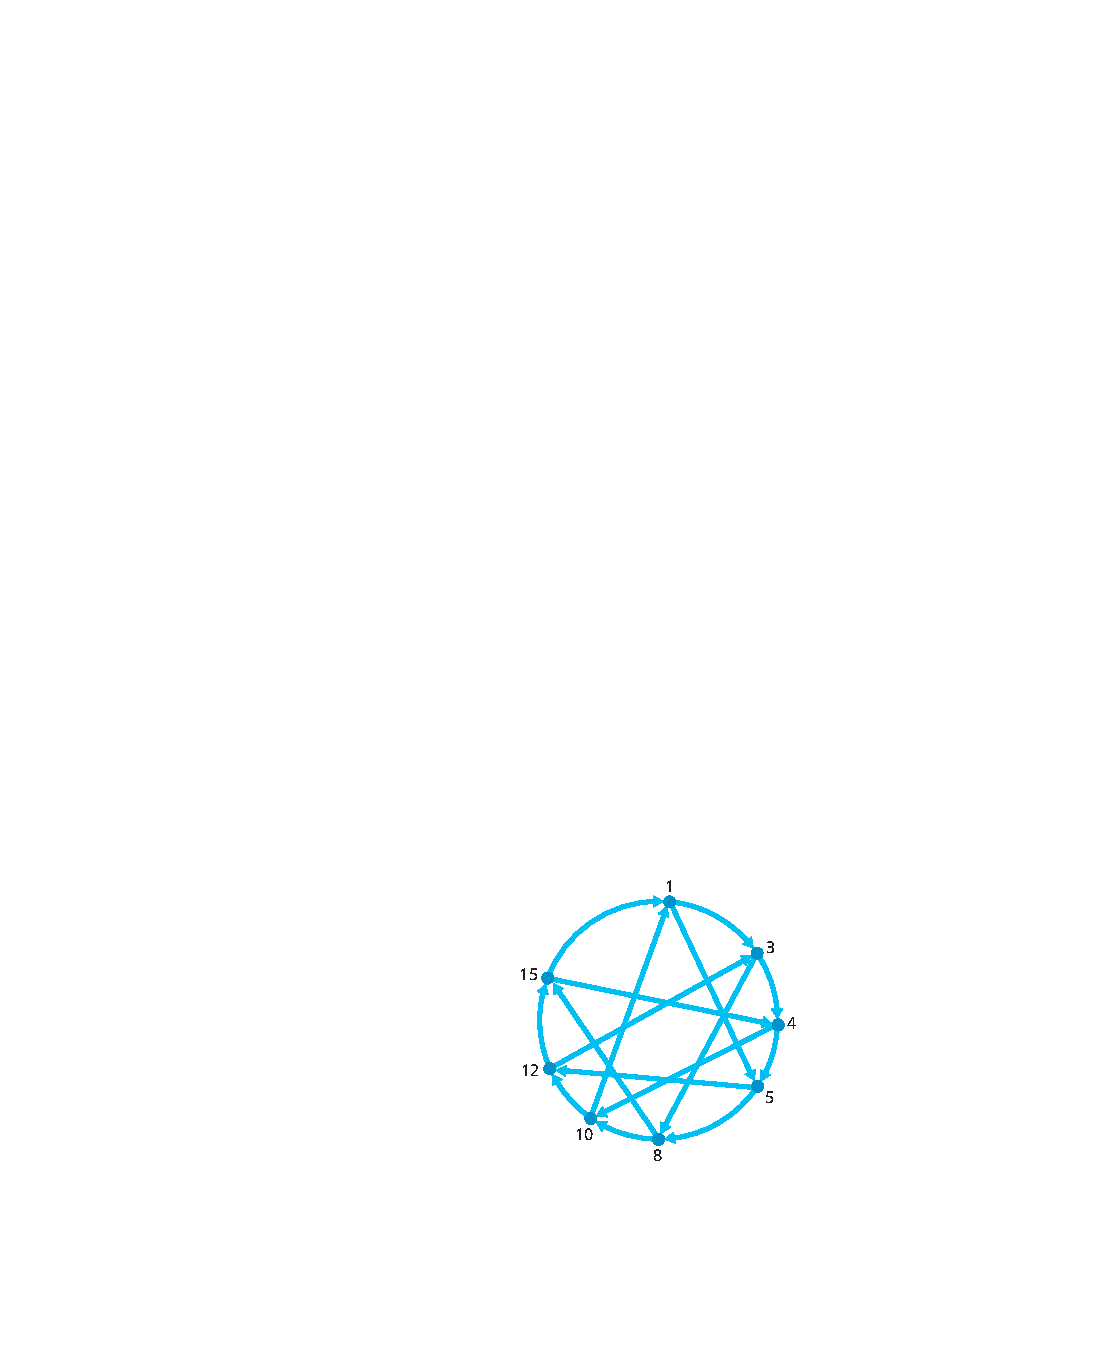
\includegraphics[width=10cm,pagebox=cropbox,clip]{CircularDHTWithShortcuts.pdf}
 \caption{ショートカット付き円形DHT}
 \label{fig:circular_dht_with_shortcuts}
\end{figure}

\subsubsection{ピアチャーン}
またP2Pにおいてピアがトレントから自由に参加や離脱が可能という点をDHTの設計において考慮が必要である.これをピアチャーンと呼ぶ.離脱時にその次にピアの情報を取得し,円形DHTを保持することである.例えば図\ref{fig:circular_dht}においてピア5が離れた時にピア4はピア8の情報を保持しているのでピア8にピア10の情報を請求し,ピア4の保持している情報に加える.これにより,ピアの自由な参加離脱に対応ができるようになる.
\\

\section{ソケットプログラミング}
ソケット API(Socket Application Programming Interface)は,アプリケーションに対して,異なるホスト間での通信をサポートするためのトランスポート層以下の機能を提供するプログラミングインタフェースで,クライアント/サーバモデルを実現するために用いられるものである.


 

\end{document}
